\documentclass[11pt,a4paper]{article}
% ---------------------------------------------------------------------
%  TFPT --- Horizon and black-hole readouts of the seam constant c_3
%  Hawking/de Sitter/Unruh thermality, BH thermodynamics, Page, scrambling,
%  Nariai bound, turnaround radius, GW speed, birefringence. Honest typing.
% ---------------------------------------------------------------------
\usepackage[T1]{fontenc}
\usepackage[utf8]{inputenc}
\usepackage[english]{babel}
\usepackage{lmodern}
\usepackage[a4paper,margin=2.3cm]{geometry}
\usepackage{amsmath,amssymb,amsthm,mathtools}
\usepackage{booktabs,array,tabularx}
\usepackage{enumitem}
\usepackage{xcolor}
\usepackage[most]{tcolorbox}
\usepackage{microtype}
\usepackage[hidelinks,colorlinks=true,linkcolor=blue!55!black,urlcolor=blue!55!black]{hyperref}
\emergencystretch=3em

\definecolor{tfblue}{HTML}{1F4E79}
\definecolor{tfgreen}{HTML}{1E7B45}
\definecolor{tfred}{HTML}{9B2226}
\definecolor{tfgold}{HTML}{B8860B}

\newtcolorbox{keybox}[1][]{enhanced,breakable,colback=tfblue!5!white,colframe=tfblue,fonttitle=\bfseries,coltitle=white,title={#1}}
\newtcolorbox{winbox}[1][]{enhanced,breakable,colback=tfgreen!6!white,colframe=tfgreen!75!black,fonttitle=\bfseries,coltitle=white,title={#1}}
\newtcolorbox{gapbox}[1][]{enhanced,breakable,colback=tfred!5!white,colframe=tfred!80!black,fonttitle=\bfseries,coltitle=white,title={#1}}

% --- six-grade status markers ---
\newcommand{\tI}{{\small\textcolor{tfgreen}{\textbf{[I]}}}}
\newcommand{\tL}{{\small\textcolor{tfblue}{\textbf{[L]}}}}
\newcommand{\tF}{{\small\textcolor{tfgreen!45!black}{\textbf{[F]}}}}
\newcommand{\tN}{{\small\textcolor{tfgreen}{\textbf{[N]}}}}
\newcommand{\tP}{{\small\textcolor{tfgold}{\textbf{[P]}}}}
\newcommand{\tA}{{\small\textcolor{tfred}{\textbf{[A]}}}}
% inline reference to the script that machine-checks a claim (see verification/)
\newcommand{\veri}[1]{\,{\footnotesize\textcolor{tfblue!70!black}{[\,\texttt{verification/#1}\,]}}}
\newcommand{\cthree}{c_3}
\newcommand{\Mbar}{\bar M_{\mathrm{Pl}}}
\newcommand{\ainv}{\alpha^{-1}_\star}
\newcommand{\Z}{\mathbb{Z}}
\newcommand{\Nfam}{N_{\mathrm{fam}}}
\setlist{itemsep=2pt,topsep=3pt}
\newcolumntype{Y}{>{\raggedright\arraybackslash}X}

\title{\vspace{-1.2cm}\textbf{TFPT --- Appendix H: the horizon unit system}\\[2mm]
\large One seam constant $\cthree=\tfrac1{8\pi}$ as the universal horizon thermal code\\
(Hawking, de Sitter, Unruh, Page, scrambling --- \emph{standard physics in seam units, not new gravity})}
\author{}\date{\today}

\begin{document}
\maketitle
\vspace{-0.6cm}

\begin{keybox}[What this document is about]
A change of bookkeeping, not new gravitational physics: if gravity is the geometry-channel readout of the
seam, then \emph{all} horizons read the same boundary constant $c_3=\tfrac1{8\pi}$. This note collects the
readouts --- Hawking, de Sitter and Unruh temperature, black-hole thermodynamics, the Page time,
scrambling, the Nariai bound, $v_{\mathrm{GW}}=c$ and cosmic birefringence --- in seam units, with two
genuine compiler fingerprints ($1920=|W(D_5)|$, $|\mu_4|=4$).
\end{keybox}

\begin{keybox}[The TFPT document set --- what is treated where]
\textbf{Plain language:} TFPT is a small discrete compiler. Two inputs --- the seam constant
$c_3=\tfrac1{8\pi}$ and the carrier rank $g_{\mathrm{car}}=5$ --- build $D_5\oplus A_3+\mu_4\Rightarrow E_8$
and read off the Standard Model, the constants and the scale grammar. The development is \textbf{five short
documents plus this appendix}, best read in order:
\begin{enumerate}[leftmargin=1.7em,itemsep=1pt]
\item \texttt{introduction} --- reading guide, compiler closure, paper-by-paper comparison, predictions, the dependency DAG and proof ledger.
\item \texttt{tfpt\_1\_architecture\_e8} --- the two axioms, the derivation map, the EM fixed point $\alpha^{-1}$, the $D_5\oplus A_3+\mu_4\Rightarrow E_8$ construction.
\item \texttt{tfpt\_2\_standard\_model} --- the SM in one $\varphi_0$-ladder formula, flavor from parabolic transport, the worked closures, and gravity/QG as the seam response.
\item \texttt{tfpt\_3\_e8\_audit\_bootstrap} --- the seven $E_8$ slices as an audit raster, the cascade bridge, the M\"obius bootstrap.
\item \texttt{tfpt\_4\_frontier} --- honest status of $\eta_B$, $m_p/m_e$, Koide, dark matter, full QG.
\item[H.] \texttt{tfpt\_horizon\_readouts} --- \textbf{Appendix H}: one seam constant as the universal horizon thermal code (a unit-system reframe, \emph{not} a peer paper, \emph{not} new physics).
\end{enumerate}
\textbf{You are reading Appendix H} --- a notation/unit reframing; all new-physics content lives in documents 1--4.
\end{keybox}

\tableofcontents
\bigskip

\begin{keybox}[Scope and honest typing]
If gravity is the geometry-channel readout of the seam (companion note ``Seam response grammar''), then
horizons are not separate miracles --- they all read the \emph{same} boundary normaliser $\cthree=1/(8\pi)$.
This note collects the readouts. Markers: \tP\ standard horizon physics rewritten in TFPT/seam units (no
new claim), \tI\ an exact compiler connection (audit-level), \tN\ a numerical readout (reproduced),
\tA\ a search target, not a result. Nothing
here is sold as new gravitational physics; it is a \emph{change of bookkeeping} that exposes shared
structure.
\end{keybox}

\begin{keybox}[Unit conventions used throughout]
Three unit systems appear; the seam factor $\cthree=1/(8\pi)$ is the same number in all of them, only the
carried dimensionful constants change:
\begin{center}\small
\renewcommand{\arraystretch}{1.25}
\begin{tabularx}{\linewidth}{@{}p{3.4cm}p{4.3cm}Y@{}}
\toprule
\textbf{system} & \textbf{convention} & \textbf{Hawking temperature} \\
\midrule
Planck & $G{=}\hbar{=}c{=}k_B{=}1$ & $T_H=\cthree/M=1/(8\pi M)$ \\
reduced Planck & $\Mbar=M_{\rm Pl}/\sqrt{8\pi}$, $\hbar{=}c{=}k_B{=}1$ & $T_H=\cthree\,\Mbar^2/M$ \\
SI & restore $G,\hbar,c,k_B$ & $T_H=\dfrac{\hbar c^3}{8\pi G k_B M}=\cthree\,\dfrac{\hbar c^3}{Gk_BM}$ \\
\bottomrule
\end{tabularx}
\end{center}
All boxed formulas below are in Planck units unless stated; the seam constant is dimensionless.
\end{keybox}

\medskip
\noindent\emph{Standard references for the formulas reframed here:} Hawking temperature and radiation
(Hawking 1975); Bekenstein--Hawking entropy (Bekenstein 1973, Hawking 1975); Page time (Page 1993);
fast scrambling $t_{\rm scr}\sim\beta\log S$ (Sekino--Susskind 2008, Maldacena--Shenker--Stanford 2016);
Nariai bound (Nariai 1950); de Sitter thermodynamics (Gibbons--Hawking 1977). \emph{Nothing below is a
new derivation of these} --- only a rewriting in the seam unit $\cthree$.

% =====================================================================
\section{The seam constant is the universal horizon temperature factor}
% =====================================================================
Every Killing horizon has $T=\hbar\kappa/(2\pi c k_B)$. Since
\[
  \boxed{\ \frac{1}{2\pi}=4\cthree,\qquad \frac{1}{8\pi}=\cthree\ }\qquad\tI,
\]
the universal factor \emph{is} the seam constant: $T_{\mathrm{hor}}=4\cthree\,\hbar\kappa/(ck_B)$. Black
holes, de Sitter and Unruh therefore share \emph{one} thermal grammar. \tP\ \veri{v8\_horizon.py}

% =====================================================================
\section{Schwarzschild thermodynamics in four $\cthree$-lines}
% =====================================================================
For a non-rotating, uncharged hole in Planck units ($G{=}\hbar{=}c{=}k_B{=}1$):
\[
  \boxed{\ T_H=\frac{\cthree}{M},\qquad S_{BH}=\frac{M^2}{2\cthree},\qquad
  P_H=\frac{\cthree}{1920\,M^2},\qquad \tau_{\mathrm{evap}}=\frac{640}{\cthree}M^3\ }\qquad\tP.
\]
Two of the constants are compiler numbers, not coincidences:
\begin{itemize}\setlength\itemsep{2pt}
\item the Hawking temperature factor is $\cthree=1/(8\pi)$ --- the same P1 boundary normaliser; \tI
\item the radiated-power denominator is $1920=|W(D_5)|$, the Weyl-group order of the $D_5$ carrier. \tI
\end{itemize}
\noindent\emph{Scope of $P_H$:} this is the idealised massless single-channel blackbody normalisation.
Greybody factors and the radiated species content shift the phenomenological evaporation coefficient; the
$\cthree$-form is the convention statement, not a general phenomenological prediction.

\begin{center}\small
\renewcommand{\arraystretch}{1.2}
\begin{tabularx}{\linewidth}{@{}p{4.2cm}YY@{}}
\toprule
\textbf{object} & \textbf{$T_H$} & \textbf{lifetime / entropy} \\
\midrule
solar-mass hole & $6.17\times10^{-8}$ K & $\tau_{\mathrm{evap}}\approx2.1\times10^{67}$ yr; $S/k_B\approx1.05\times10^{77}$ \\
PBH evaporating now ($1.7\times10^{11}$ kg) & $k_BT\approx61$ MeV & relevant for $\gamma$/$\nu$ PBH signatures \\
\bottomrule
\end{tabularx}
\end{center}

% =====================================================================
\section{Page time and scrambling}
% =====================================================================
Since $S_{BH}\propto M^2$ and $\tau\propto M^3$, the Page point ($M\to M/\sqrt2$) is
\[
  t_{\mathrm{Page}}=\Bigl(1-\tfrac1{2\sqrt2}\Bigr)\tau_{\mathrm{evap}}\approx0.6464\,\tau_{\mathrm{evap}}\qquad\tP.
\]
In TFPT the Page curve is \emph{boundary recoverability}: the physical sector is OS-reconstructed and
gapped, and the recovered mutual information decays at the transfer rate,
$I(A{:}C|B)_n\sim\lambda_2^{\,n}=(2/3)^{6n}$. \textbf{This is the same operator that builds the Standard
Model:} the boundary transport spectrum is $\{1,(2/3)^6,(1/3)^6\}$ and its sub-leading eigenvalue
$\lambda_2=(2/3)^6$ is exactly the flavor-gap eigenvalue of Paper~2 ($\Delta_{\mathrm{gap}}=-\log(2/3)^6=6\log\tfrac32$).
One boundary transport thus governs \emph{both} the SM flavor hierarchy and the horizon information recovery.
\tI\ \veri{v54\_seam\_horizon\_keystones.py} The scrambling prefactor carries a $\mu_4$ signature: with
$\beta=1/T_H=8\pi M$, $\beta/2\pi=4M$, so
\[
  \boxed{\ t_{\mathrm{scr}}\sim|\mu_4|\,M\log S\ }\qquad(|\mu_4|=4)\qquad\tI\text{-audit}.
\]

% =====================================================================
\section{De Sitter and the Nariai bound from the $\Lambda$ closure}
% =====================================================================
With the action-grammar Hubble/$\Lambda$ readouts ($H_0/\Mbar=e^{-\ainv}/(2\pi\sqrt{\Omega_\Lambda})$,
$\rho_\Lambda/\Mbar^4\sim e^{-2\ainv}$), the asymptotic de Sitter horizon gives
\[
  \boxed{\ \frac{T_{dS}}{\Mbar}=16\cthree^2\,e^{-\ainv},\qquad
  S_{dS}=\frac{e^{2\ainv}}{128\cthree^4}=32\pi^4 e^{2\ainv}\approx3.32\times10^{122}\ }\qquad\tP.
\]
This is the area-law horizon capacity of the universe from $(\ainv,\cthree,H_\Lambda)$ alone. The maximal
black hole in de Sitter (Nariai) is
\[
  M_N\approx2.16\times10^{22}\,M_\odot\approx4.3\times10^{52}\,\mathrm{kg},\qquad S_N=\tfrac13 S_{dS}\qquad\tP,
\]
the absolute gravitational-capacity limit, not an observed structure.

% =====================================================================
\section{The maximal black hole is the anchor: SdS in seam units}
% =====================================================================
The Nariai limit is not just a capacity number --- written in compiler units, the entire
Schwarzschild--de~Sitter (SdS) family lands on atoms that are already load-bearing elsewhere in TFPT,
with no adjustable parameter on either side. \tI\ \veri{v101\_horizon\_anchor.py}

\begin{keybox}[Nariai $=$ the anchor; the Koide $2/3$ is the entropy bound \tI\ (\veri{v101\_horizon\_anchor.py})]
With $f(r)=1-2M/r-\Lambda r^2/3$, the horizon cubic at the maximal mass
$M_N=1/(3\sqrt\Lambda)=1/(N_{\mathrm{fam}}\sqrt\Lambda)$ is, in units $1/\sqrt\Lambda$,
\[
  \boxed{\ t^3-3t+2=(t-1)^2(t+2)\ }\qquad\text{roots }(1,1,-2),
\]
with coefficients $(-3,2)=(-N_{\mathrm{fam}},|\Z_2|)$ --- and the root pattern is exactly the
\textbf{traceless projection of the anchor}: $a-\tfrac{p_1(a)}{3}\mathbf 1=-\tfrac13(1,1,-2)$ for
$a=(1,1,2)$ (compare $\chi_a=(t-1)^2(t-2)$, Paper~1). Five exact companions:
\begin{itemize}\setlength\itemsep{2pt}
\item \textbf{Entropy bound $=$ the Koide branch value.} Each Nariai horizon carries $S_{dS}/3=S_{dS}/N_{\mathrm{fam}}$
and the total is $\boxed{S_{\mathrm{Nariai}}/S_{dS}=2/3=|\Z_2|/N_{\mathrm{fam}}}$ (deficit exactly $S_{dS}/3$). The
interpolation in $x=r_b/r_c$ is the closed form
$S_{\mathrm{tot}}/S_{dS}=(x^2{+}1)/(x^2{+}x{+}1)$ --- denominator $=\Phi_3(x)$, the $N_{\mathrm{fam}}$
cyclotomic --- monotone from $1$ to $2/3$ with its minimum exactly at the merge (Fig.~\ref{fig:nariai}a).
\item \textbf{Three-sheet conservation.} The cubic is traceless with fixed $e_2$, so
$\pi\sum_i r_i^2=6\pi/\Lambda=|\Z_2|\,S_{dS}$ for \emph{every} $M$: the black hole redistributes entropy
between the two physical sheets and the virtual third root; the three-sheet total never moves.
\item \textbf{Koide-form quotient of the roots.} $Q_{\mathrm{geom}}=\sum r_i^2/(\sum|r_i|)^2$ runs
monotonically over $[\tfrac38,\tfrac12]$: pure dS gives $\tfrac12=|\Z_2|/|\mu_4|=\delta$ (the half-step),
Nariai gives $\tfrac38=p_2(a)/e_1(a)^2$ --- exactly the two nonzero $SU(4)_1$ conformal weights
(Fig.~\ref{fig:nariai}b).
\item \textbf{The mass line is a double cover.} $\operatorname{disc}_r\propto(1-3m)(1+3m)$ in
$m=M\sqrt\Lambda$: branch points $m=\pm1/N_{\mathrm{fam}}$, separation $2/3=|\Z_2|/N_{\mathrm{fam}}$, deck involution
$=$ the black-hole$\,\leftrightarrow\,$cosmological horizon swap --- the gravitational twin of the flavor
sheet $\Z_2$ and of the split $N_{\mathrm{fam}}$-linear cover $(3x{+}2)(3x{+}5)$ of Paper~2 (Fig.~\ref{fig:sdscover}).
\item \textbf{Temperature lemma / orientation.} $|\kappa_b/\kappa_c|=(2x{+}1)/(x(x{+}2))>1$ for $x<1$
(equality iff $x=1$): the black-hole sheet is \emph{always} hotter, so evaporation flows \emph{away} from
the merge --- the anchor configuration is the \textbf{repeller} and the democratic endpoint the attractor,
the same orientation as the flavor flow (Koide attractor / carrier repeller, Paper~4). \emph{Audit reading.}
\end{itemize}
Completing the seam-unit table: $dM=\cthree\,\kappa\,dA$ (first law), $M=2\cthree\,\kappa A$ (Smarr),
$S\le ER/(4\cthree)$ (Bekenstein), $P_H=\cthree/(1920\,M^2)$, lifetime
$\tau=5120\pi M^3=128\,g_{\mathrm{car}}M^3/\cthree$ ($128=2^7$ the dS prefactor, $7$ the scalaron exponent;
photon/geometric-optics conventions, typed external), Kerr $A_{\mathrm{ext}}=M^2/\cthree$ with
$A_{\mathrm{ext}}/A_{\mathrm{Schw}}=1/2=1/|\Z_2|$ and $S_{\mathrm{ext}}=M^2/(4\cthree)$, and the
Bekenstein--Mukhanov--Hod area quantum $4\ln3=\ln81=\ln(N_{\mathrm{fam}}^4)=\ln(\operatorname{disc}$ of the flavor
cover$)$ (\tP\ as the QNM reading). \emph{Honest scope:} the GR identities are textbook facts; the \tI\
content is six independent landings on already-load-bearing atoms with zero free parameters. The
``carrier in the bulk'' reading (two glue chiralities $=$ two horizon sheets, ramification $=$ Nariai)
stays \tP. No new data test ($M_N$ today $\sim10^{22}M_\odot$): a structure surface, not a measurement
surface.
\end{keybox}

\begin{figure}[h]
\centering
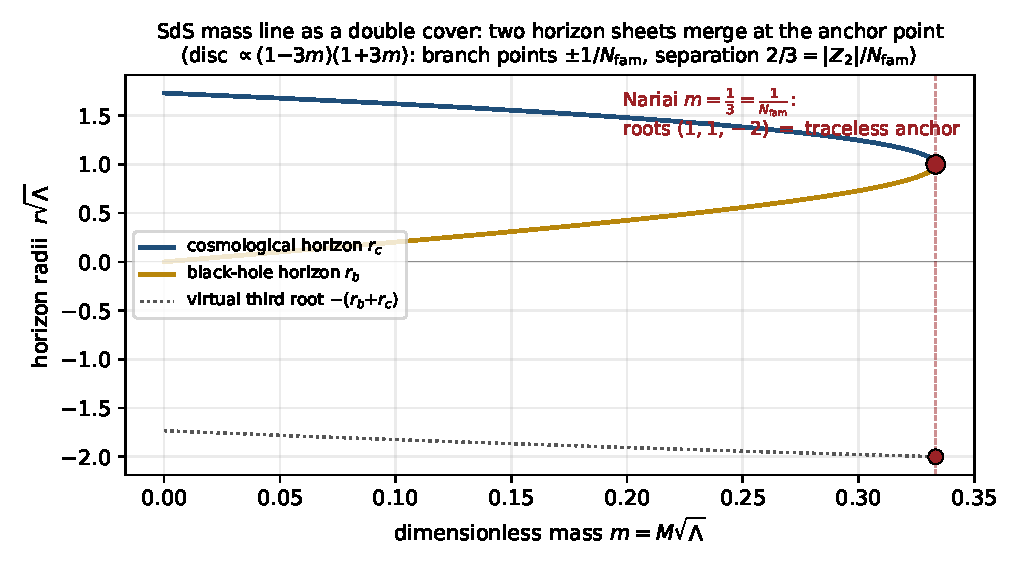
\includegraphics[width=0.78\linewidth]{figures/sds_cover.pdf}
\caption{The SdS mass line as a double cover: black-hole and cosmological horizon sheets merge at the
Nariai point $m=1/N_{\mathrm{fam}}$, where the three roots form the traceless anchor pattern $(1,1,-2)$.
\veri{v101\_horizon\_anchor.py}}
\label{fig:sdscover}
\end{figure}

\begin{figure}[h]
\centering
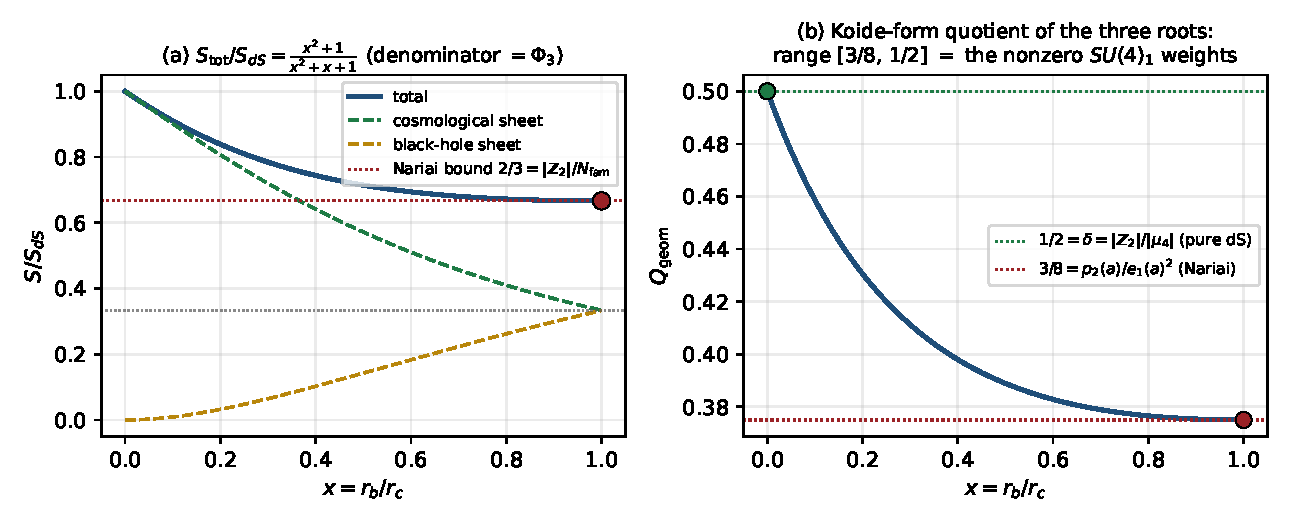
\includegraphics[width=0.94\linewidth]{figures/nariai_entropy.pdf}
\caption{(a) Total SdS entropy interpolates from $S_{dS}$ to the Nariai bound $\tfrac23 S_{dS}$ via
$(x^2{+}1)/\Phi_3(x)$. (b) The Koide-form quotient of the three roots runs exactly over the nonzero
$SU(4)_1$ weights $[\tfrac38,\tfrac12]$. \veri{v101\_horizon\_anchor.py}}
\label{fig:nariai}
\end{figure}

\begin{figure}[h]
\centering
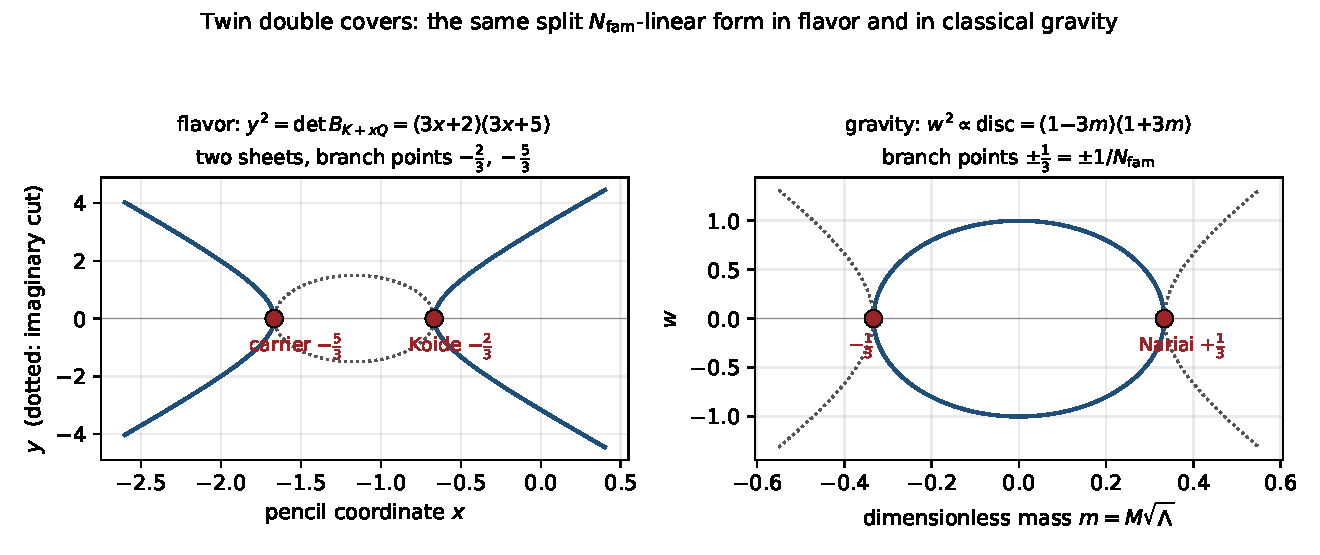
\includegraphics[width=0.94\linewidth]{figures/cover_twins.pdf}
\caption{Twin double covers: the flavor anchor-block cover $y^2=(3x{+}2)(3x{+}5)$ (Paper~2) and the SdS
mass-line cover $w^2\propto(1{-}3m)(1{+}3m)$ share the split $N_{\mathrm{fam}}$-linear form with rational
branch points at spine-over-family values. \veri{v101\_horizon\_anchor.py}}
\label{fig:covertwins}
\end{figure}

\begin{winbox}[One orientation: the anchor is the \emph{stationary repeller} in both sectors \tI/\tP\ (\veri{v102\_seam\_orientation.py})]
The evaporation direction of the temperature lemma upgrades to exact variational structure on both
one-dimensional moduli lines (Fig.~\ref{fig:orientation}). \textbf{Flavor:} the canonical relaxation
$\dot q=(\Delta/N_{\mathrm{fam}})(q{-}2)(q{-}5)$ is the \emph{gradient flow} of the cubic potential
\[
  V(q)=-\frac{\Delta}{N_{\mathrm{fam}}}\Bigl(\frac{q^3}{3}-\frac{7}{2}q^2+10q\Bigr),\qquad
  \boxed{\ V''(2)=+\Delta,\quad V''(5)=-\Delta\ }
\]
--- the critical points are exactly the two branch points, the stationary curvatures are $\pm$the
transfer gap, the inflection sits at $q=\tfrac72=$ scalaron$/2$, and the Lyapunov rate is constant:
$d(-\ln\rho)/dt=\Delta$ exactly. \textbf{Gravity:} the SdS entropy functional has
\[
  \frac{d}{dx}\frac{S_{\mathrm{tot}}}{S_{dS}}=\frac{(x-1)(x+1)}{\Phi_3(x)^2},\qquad
  \boxed{\ \Bigl(\frac{S_{\mathrm{tot}}}{S_{dS}}\Bigr)''(1)=\frac29=\frac{|\Z_2|}{N_{\mathrm{fam}}^2}=\frac23\cdot\frac13\ }
\]
--- the Nariai/anchor point is the \emph{unique} physical stationary point, its curvature is a grammar
constant ($=$ the product of the two Nariai entropy fractions), and the temperature lemma makes the
evaporation an entropy \emph{ascent} away from it. \textbf{Orientation theorem \tI:} in both sectors the
anchor-type configuration is a stationary point of the natural functional and the dynamics flows away
from it, with grammar-constant stationary curvatures. \emph{Honest disanalogies (recorded):} the flavor
attractor is itself a branch point while the gravity attractor is the smooth endpoint; the flavor
functional is the potential of a \tP-typed relaxation while the gravity functional is the
Bekenstein--Hawking entropy --- ``one variational principle of the seam'' stays a \emph{reading} \tP, and
no open gate is touched.
\end{winbox}

\begin{figure}[h]
\centering
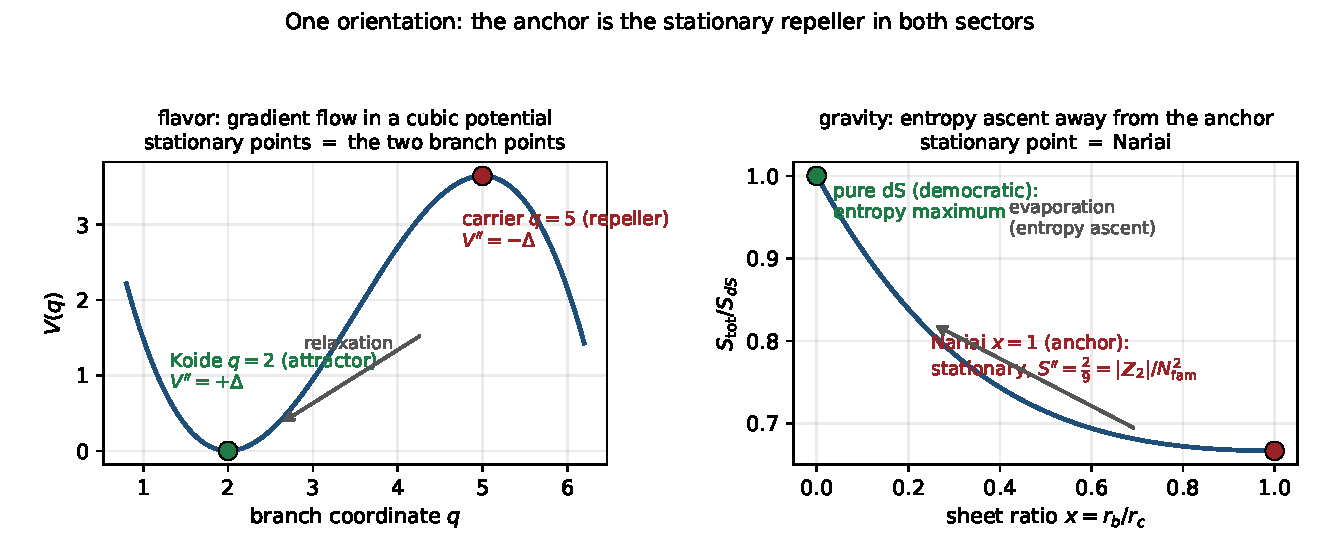
\includegraphics[width=0.94\linewidth]{figures/orientation.pdf}
\caption{The orientation theorem: the anchor configuration is the stationary repeller of the natural
functional in both sectors --- flavor (cubic potential, curvatures $\pm\Delta$) and gravity (SdS entropy,
curvature $2/9=|\Z_2|/N_{\mathrm{fam}}^2$). \veri{v102\_seam\_orientation.py}}
\label{fig:orientation}
\end{figure}

\begin{keybox}[The trisection normal form: the canonical coordinate exists \tI\ (\veri{v103\_trisection\_normal\_form.py})]
The curvature-matching question of the previous box has a closed answer. The SdS horizon cubic is
uniformized by \textbf{angle trisection}: with $r=2\cos\theta$ (units $1/\sqrt\Lambda$),
$r^3-3r=2\cos3\theta$ \emph{exactly}, so the cubic is $\cos3\theta=-3m$ --- the three horizon roots are
the three trisection branches (the $\Z_3$ rotation $=$ the triality deck, cf.\ $\operatorname{coker}Q=\Z/\Nfam$).
In the centered angle $\psi$ ($\cos\varphi=-3m$, $\psi=\varphi-\pi$; Nariai $\psi=0$, pure dS $\psi=\pi/2$,
deck $\psi\to-\psi$):
\[
  m=\frac{\cos\psi}{\Nfam},\qquad
  \boxed{\ \frac{S_{\mathrm{tot}}}{S_{dS}}=\frac43-\frac23\cos\frac{2\psi}{3}\ }
\]
--- \emph{one} cosine whose mean ($|\mu_4|/\Nfam$), amplitude and frequency (both $|\Z_2|/\Nfam$) are glue
atoms over the family count (Fig.~\ref{fig:trisection}). Three exact consequences:
\begin{itemize}\setlength\itemsep{1pt}
  \item \textbf{Canonical curvature $=$ the Koide constant to the family power:}
  $\sigma''(\psi{=}0)=\tfrac{8}{27}=(\tfrac23)^3=(|\Z_2|/\Nfam)^{\Nfam}$.
  \item \textbf{Invariant base slope:} $d\sigma/dm|_{\mathrm{Nariai}}=-\tfrac89=-\operatorname{rank}E_8/\Nfam^2$
  (coordinate-invariant, cross-checked in both coordinates; generally $-\tfrac43\sin(2\psi/3)/\sin\psi$);
  dimensionful $dS_{\mathrm{tot}}/dM|_N=-r_N/(\Nfam\cthree)$.
  \item \textbf{The bridge:} the flavor invariant is a \emph{rate}, multiplier $(2/3)^6=(2/3)^{2\Nfam}$
  per transport step; the gravity invariant is a \emph{curvature}, $(2/3)^{\Nfam}$ in the canonical angle
  --- same base $2/3=|\Z_2|/\Nfam$, exponent ratio $2=|\Z_2|$. What is still missing for a full
  identification is the gravity-side \emph{clock} (the near-Nariai evaporation generator that converts
  curvature into a rate) --- the same class of missing object as the Koide transfer generator of Paper~4:
  \textbf{one clock, two known geometries}. That identification stays \tP.
\end{itemize}
\end{keybox}

\begin{figure}[h]
\centering
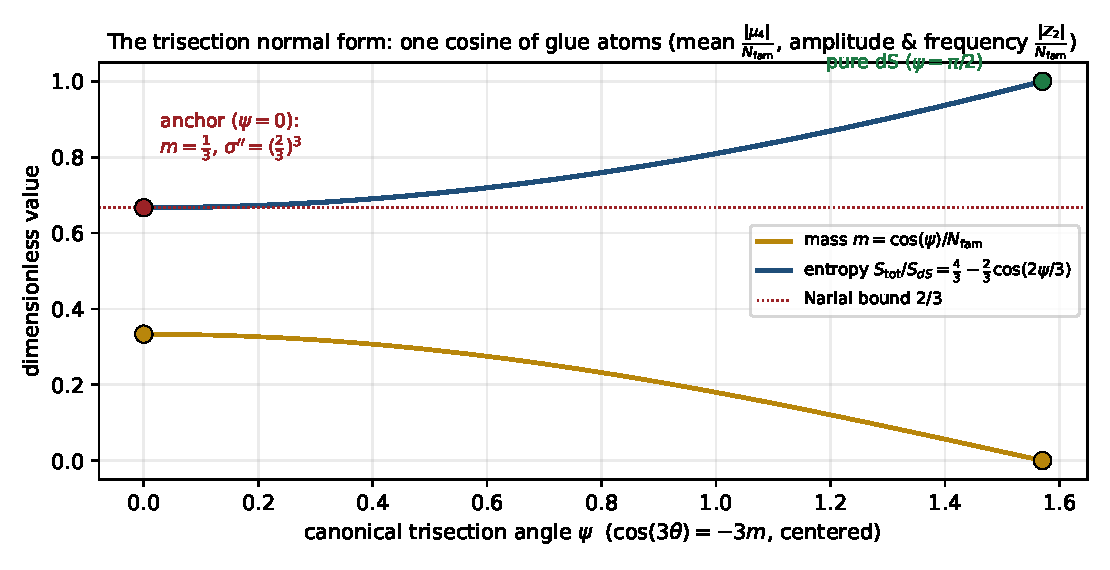
\includegraphics[width=0.86\linewidth]{figures/trisection.pdf}
\caption{The trisection normal form: in the canonical angle $\psi$ the mass and the total entropy are
pure (co)sines built from glue atoms; the anchor sits at $\psi=0$ with canonical curvature
$(2/3)^3$. \veri{v103\_trisection\_normal\_form.py}}
\label{fig:trisection}
\end{figure}

\begin{winbox}[The classical clock speaks anchor --- and the honest $(2/3)$-test \tI/\tP\ (\veri{v104\_nariai\_clock.py})]
The clock question of the previous box has a \emph{classical} half, and it is pure GR
(Ginsparg--Perry~1983; Bousso--Hawking class): linearize around the Nariai geometry
$dS_2\times S^2$. \textbf{Static pin \tI:} on the $dS_2$ static patch the function $\phi(\rho)=\rho$
satisfies $\frac{d}{d\rho}\bigl[(1-\Lambda\rho^2)\phi'\bigr]=-2\Lambda\phi$ \emph{exactly} --- and this
static mode \emph{is} the exact SdS two-horizon deformation, so the $S^2$-radius modulus mass is pinned
internally: $m^2=-2\Lambda=-|\Z_2|\Lambda$ (the Laplace-type form of the linearization is the one
external GR import, typed honestly). The Euclidean spectrum is the Ginsparg--Perry tower
$(l(l+1)-2)\Lambda$: exactly \emph{one} negative mode $-|\Z_2|\Lambda$. \textbf{The clock \tI:} in
Hubble units the homogeneous modes $\phi\sim e^{\lambda Ht}$ obey
\[
  \boxed{\ \chi_{\mathrm{clock}}(\lambda)=\lambda^2+\lambda-2=(\lambda-1)(\lambda+2)\ }
\]
--- \textbf{the anchor quadratic}: eigenvalues $\{1,-2\}$ $=$ the distinct anchor roots, and the Nariai
cubic factors as $(t-1)^2(t+2)=(t-1)\cdot\chi_{\mathrm{clock}}(t)$. The anchor thus appears a
\emph{third} time: as configuration roots, as the curvature base, and as the spectrum of the linearized
clock. The horizon split is linear in the canonical angle with coefficient $1/\sqrt{\Nfam}$, and the
entropy deviation grows at exactly $2H=|\Z_2|\times$Hubble. \textbf{Honest $(2/3)$-test \tP:} the
classical clock eigenvalues are \emph{integers}, not $(2/3)$-powers --- the $(2/3)$-powers stay in the
functional (curvature $(2/3)^{\Nfam}$). The conversion curvature$\to$rate at one loop (quantum
(anti-)evaporation) remains external QFT input: the bridge to the flavor rate $(2/3)^{2\Nfam}$ is
\emph{not} closed here. The seam variational principle now has exactly \emph{one} missing object: the
quantum clock.
\end{winbox}

\begin{winbox}[The quantum-clock target, made quantitative \tI/\tP\ (\veri{v107\_quantum\_clock\_target.py})]
Instead of guessing the quantum clock, its job description can be pinned exactly. \textbf{(1) The
classical clock already lives on the cusp ladder \tI:} across the physical Ginsparg--Perry modes
($l=0$: $(\lambda{-}1)(\lambda{+}2)$; $l=1$: $\lambda(\lambda{+}1)$) the decay exponents are
\[
  \boxed{\ \{0,-1,-2\}=-\operatorname{Spec}(V)=-\Nfam\times\text{cusp weights}\ }
\]
--- exactly the grading that carries the transfer operator's eigenspaces (Papers~2/6); the $l\ge2$ modes
are damped oscillations with $\operatorname{Re}\lambda=-\tfrac12=-\delta$ (audit). \textbf{(2) The exact
target \tI:} the transfer rates $\{0,\Delta,6\ln3\}$ are \emph{not} weight-linear ---
$\mathrm{rate}(2)/\mathrm{rate}(1)=\log_{3/2}3=1+\log_{3/2}2=2.7095$, with the exact identity
$(1/3)^6=\bigl((2/3)^6\bigr)^{\log_{3/2}3}$: \emph{the quantum clock must bend the weight-linear spectrum
by $\log_{9/4}3=1.35476$ per weight step}. \textbf{(3) Coupling landscape \tI:} the dimensionless clock
coupling $\kappa=(c/24\pi)(\Lambda/\bar M_{\mathrm{Pl}}^2)$ with $c=8$ is $7.6\times10^{-122}$ at the
cosmological Nariai (hopeless) and $\kappa=1/(3\pi)=0.106$ at seam curvature --- the only regime where an
$O(0.35)$ bend is reachable, and it is borderline non-perturbative: one-loop linear response cannot fix
the bend; an $O(1)$ resummation or an exact seam construction is required. \emph{Status \tP:} R1 is
sharpened from ``find a clock'' to ``produce the bend $\log_{3/2}3$ on the cusp ladder at coupling
$O(1/3\pi)$''. Nothing is fitted; the identification stays open.
\end{winbox}

\begin{winbox}[The resummed clock: the bend has a closed form \tI/\tP\ (\veri{v124\_resummed\_clock.py})]
The ``bend'' is not an exotic target --- the frozen transfer spectrum \emph{is} a resummed logarithm.
\textbf{(1) Spectrum reading \tI:} the eigenvalues $\{1,(\tfrac23)^6,(\tfrac13)^6\}$ are exactly
\[
  \boxed{\ \lambda_n=\Bigl(1-\frac n{\Nfam}\Bigr)^{2p_2},\qquad n=0,1,2\ }
  \qquad(2p_2=6=|R^+(A_3)|),
\]
so the clock has the closed form $\mathrm{rate}(n)=-2p_2\ln(1-n/\Nfam)$ --- it reproduces
$\{0,\Delta,6\ln3\}$, and the v107 bend $\log_{3/2}3$ becomes a one-line consequence. \textbf{(2) The
linearisation carries the sheet \tI:} $\mathrm{rate}(n)=|\Z_2|\,n+\tfrac{n^2}3+\tfrac{2n^3}{27}+\cdots$
--- the one-loop term has slope exactly $|\Z_2|=2$ relative to the \emph{integer} classical
Ginsparg--Perry clock $\{0,-1,-2\}$: the quantum clock is the sheet-doubled classical clock plus the
geometric tail $\sum_k(n/N)^k/k$. \textbf{(3) The wall at $\Nfam$ \tI:} $\mathrm{rate}\to\infty$ as
$n\to\Nfam$ --- the resummed logarithm has a pole at the family count, so the cusp ladder \emph{must}
end at $n=\Nfam-1=2$: the three-level transfer spectrum is forced by the clock itself. \emph{R1
re-sharpened \tP:} the semiclassical job is now ``derive $-2p_2\ln(1-n/\Nfam)$ from the near-Nariai
one-loop at $\kappa=1/(3\pi)$'' --- a closed-form target, with the linear-response slope $|\Z_2|$ as
its first checkpoint. All spectra frozen (v54/v69/v95/v104/v107); nothing fitted.
\end{winbox}

\begin{winbox}[The clock and the wall share a spectrum \tI/\tP\ (\veri{v126\_clock\_wall\_bridge.py})]
Both ends of the resummed clock connect to established exact objects. \textbf{(1) The weights are the
parabolic weights \tI:} the arguments $n/\Nfam=\{0,\tfrac13,\tfrac23\}$ of the resummed logarithm are
\emph{exactly} $\operatorname{spec}A_0^\star$ --- the spectrum of the exact $(U_{\mathrm{wall}})$
residue (research contracts):
\[
  \boxed{\ \lambda_n=(1-\alpha_n)^{2p_2},\qquad \alpha_n\in\operatorname{spec}A_0^\star=\{0,\tfrac13,\tfrac23\}\ }
\]
--- the horizon clock and the flavor wall share their spectrum through the complement map
$\alpha\mapsto1-\alpha$. \textbf{(2) Checkpoint 1 passes classically \tI:} the clock's linear
coefficient $2p_2/\Nfam=2=|\Z_2|$ \emph{equals} the established classical entropy-deviation rate
$2H=|\Z_2|\times$Hubble (v104) --- the slope-$2$ linear response is already the classical entropy
rate; the genuinely \emph{quantum} content of R1 isolates to the geometric tail
$\sum_{k\ge2}\alpha^k/k$. \textbf{(3) The determinant is the entropy curvature \tI:}
$\det(\mathbf1-A_0^\star)=\tfrac29=|\Z_2|/\Nfam^2$ --- exactly the gravity entropy curvature at the
anchor (v102), a fourth independent appearance; $\operatorname{tr}(\mathbf1-A_0^\star)=2=|\Z_2|$,
$\det A_0^\star=0$. \emph{R1 re-targeted \tP:} derive ``rate $=-2p_2\ln(1-\alpha)$'' with $\alpha$ the
Mehta--Seshadri parabolic weight --- first order classical, tail quantum: \textbf{one spectrum, two
gates, one object $A_0^\star$}.
\end{winbox}

\begin{winbox}[The clock is a log-determinant: the tail is the ring (RPA) resummation \tI/\tP\ (\veri{v127\_ring\_resummation.py})]
The ``$O(1)$ resummation'' demanded by v107 is now \emph{typed}. For a rank-one insertion $P$
($\operatorname{tr}P^k=1$), $-\ln\det(\mathbf1-\alpha P)=-\ln(1-\alpha)=\sum_k\alpha^k/k$, so the
resummed clock is exactly
\[
  \boxed{\ \mathrm{rate}=-2p_2\,\operatorname{Tr}\ln(\mathbf1-\alpha P)\ }
\]
--- $2p_2=6$ \emph{identical} one-loop ring (RPA) towers, \textbf{one per hexagon site} ($=$ positive
root of $A_3$), with coupling $\alpha$ $=$ the parabolic weight. \emph{Ring ladder \tI:} the $k{=}1$
ring is the \emph{classical} term ($6\alpha=|\Z_2|n$, the v104/v126 entropy rate); the $k{=}2$ ring is
the first quantum correction ($\tfrac13$ at weight $1$); the partial sums converge to
$\{\Delta,6\ln3\}$ monotonically from below. \emph{Coupling cross-link \tI\ (audit):} the established
seam coupling is $\kappa=\tfrac c{24\pi}=\tfrac8{24\pi}=\tfrac1{3\pi}=\alpha_1/\pi$ --- the
\emph{first parabolic weight over $\pi$}. \emph{The wall \tI:} the ring series diverges at
$\alpha\to1$ ($n\to\Nfam$) --- the v124 wall is the standard RPA instability. \emph{R1 final form
\tP:} show that the near-Nariai one-loop effective action of the seam mode, with insertion $=$
parabolic weight and multiplicity $2p_2$, is this ring sum --- ``\textbf{the seam clock is the RPA
determinant of one mode on six sites}''. The resummation type is identified; the derivation itself
remains open.
\smallskip\\
\noindent\emph{Where the six sites live (\veri{v128\_graded\_hull.py}):} the Ginsparg--Perry $l=1$
sector --- the \emph{zero modes} $\lambda\in\{0,-1\}$ of the classical clock (v104/v107) --- has
$2l+1=3$ modes, and sheet doubling gives $2\times3=6=2p_2$ \tI: the ring multiplicity equals the
sheet-doubled zero-mode count. \tP\ reading (recorded): zero modes are exactly the modes that force
nonperturbative resummation in de Sitter one-loop physics --- the natural home of the six RPA towers.
\end{winbox}

\begin{figure}[h]
\centering
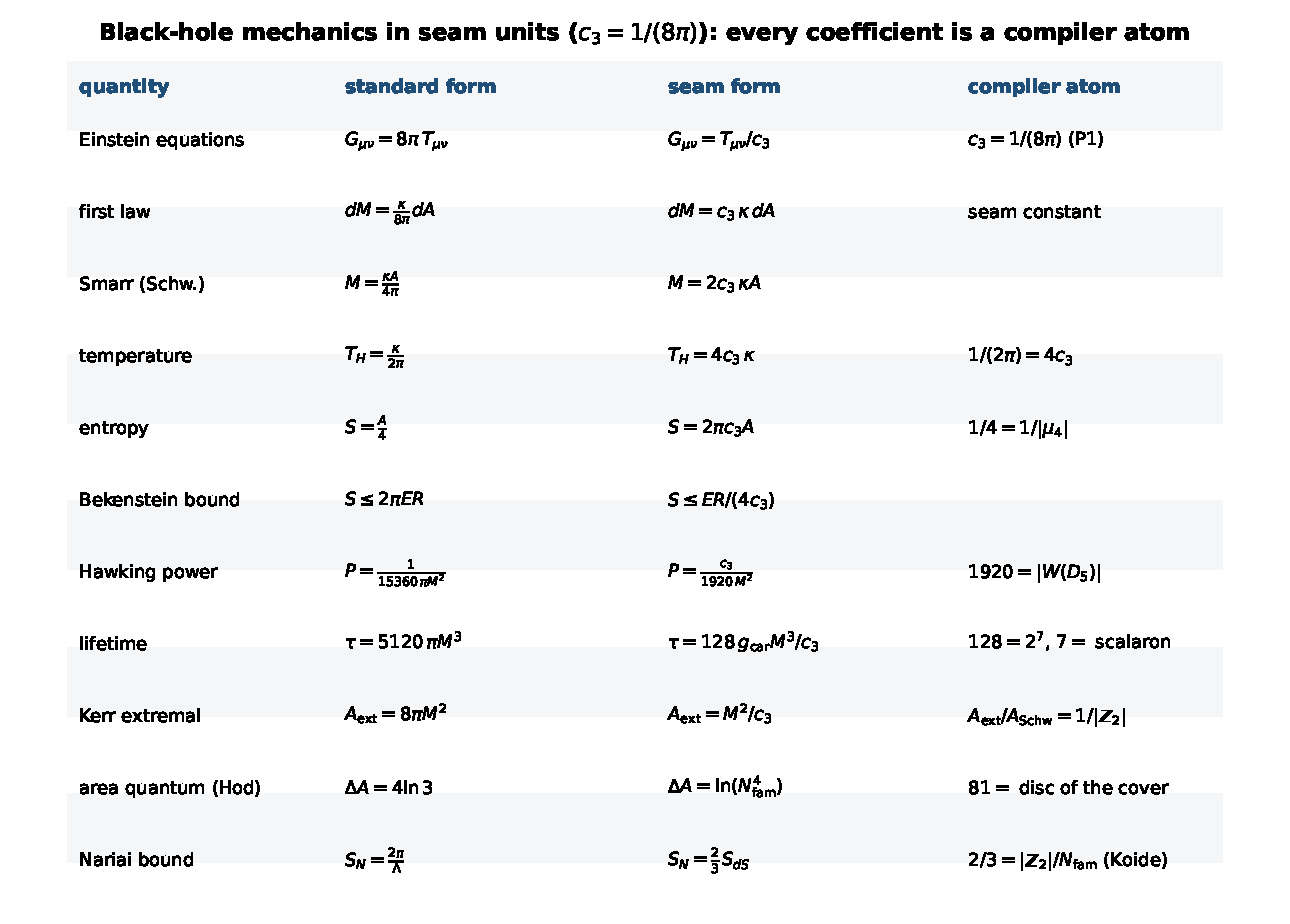
\includegraphics[width=0.9\linewidth]{figures/seam_units.pdf}
\caption{Black-hole mechanics in seam units: every classical coefficient is a compiler atom.
\veri{v101\_horizon\_anchor.py}}
\label{fig:seamunits}
\end{figure}

% =====================================================================
\section{Turnaround radius, gravitational waves, light}
% =====================================================================
\textbf{Bound structures.} In a $\Lambda$-universe the maximal bound radius is
$r_{\mathrm{ta}}(M)=\bigl(GM[\,2\pi e^{\ainv}/\Mbar]^2\bigr)^{1/3}$ --- halo, cluster, supercluster and
void scales follow from the $\Lambda$ closure with no new parameter. \tP

\textbf{Gravitational waves.} The low-curvature branch is $R+R^2$; the tensor graviton runs on the Lorentz
cone and the only extra mode (the scalaron, $M_{\mathrm{scal}}\approx3.06\times10^{13}$ GeV) is frozen for
astrophysical frequencies. Hence
\[
  \boxed{\ v_{\mathrm{GW}}=c\ }\qquad\text{(no measurable dispersion)}\qquad\tP,
\]
a clean falsifier: a genuine $v_{\mathrm{GW}}\ne c$ would break this gravity closure.

\textbf{Light.} TFPT does not predict the SI number $c$ (definitional); it predicts the \emph{universality
of the causal cone} --- RP $\to$ OS reconstruction $\to$ one Lorentzian cone shared by EM, gravity and
massless modes ($v_\gamma=v_g=c$, no native photon dispersion). What it \emph{does} compute is not a speed
shift but a polarisation rotation, cosmic birefringence
\[
  \boxed{\ \beta_{\mathrm{rad}}=\frac{u}{4\pi}\approx0.2424^\circ\ }\qquad\tN,
\]
from the same seed $u=\phi_0^{\mathrm{ret}}$ that fixes the Cabibbo angle, $\Omega_b$ and $\theta_{13}$.

% =====================================================================
\section{Search targets (not claims)}
% =====================================================================
\begin{gapbox}[Audit-level search ansätze \tA]
\begin{itemize}\setlength\itemsep{2pt}
\item \textbf{Black-hole echoes:} any near-horizon echo amplitude ratio would be a natural transfer-rate
target, $\mathcal A_{n+1}/\mathcal A_n\lesssim(2/3)^6\approx0.0878$. A search ansatz, no prediction.
\item \textbf{Quantum recovery:} the Page-curve recovery kernel $I\sim(2/3)^{6n}$ is a falsifiable shape
if a boundary-recovery rate is ever measured.
\end{itemize}
\end{gapbox}

\begin{keybox}[Net]
All horizon formulas share the one seam normalisation $1/(2\pi)=4\cthree$. Black-hole, de Sitter and Unruh
temperatures, the Page time, scrambling, the Nariai bound, turnaround radii, $v_{\mathrm{GW}}=c$ and
birefringence are \emph{readouts of one seam constant} --- standard physics rewritten in TFPT units, with
two genuine compiler fingerprints ($1920=|W(D_5)|$ in Hawking power, $|\mu_4|=4$ in scrambling). No new
gravitational physics is claimed; the value of the reframe is that horizons stop being separate modules.
\end{keybox}

% =====================================================================
\section*{Appendix: computational verification}
% =====================================================================
The seam-unit identities of this note (the thermal grammar $\tfrac1{2\pi}{=}4\cthree$, the
power denominator $1920{=}|W(D_5)|$, the de Sitter entropy form, the Page fraction, the scrambling
$|\mu_4|{=}4$, and $\beta_{\rm rad}{=}\varphi_0^{\rm ret}/4\pi{=}0.2424^\circ$) are re-derived and machine-checked in
\texttt{verification/v8\_horizon.py}. Run \texttt{python verification/v8\_horizon.py} (needs
\texttt{mpmath}); it imports the same $\cthree{=}1/(8\pi)$ primitive as the rest of the suite. The
search-target ans\"atze remain \tA\ and are deliberately not part of the pass/fail checks.

\end{document}
